\documentclass[11pt,a4paper]{article}
\usepackage[margin=24mm]{geometry}
\usepackage{fontspec}
\setmainfont{Noto Serif CJK SC}[ItalicFont={Noto Serif CJK SC},ItalicFeatures={FakeSlant=0.12}]
\setsansfont{Noto Sans CJK SC}
\setmonofont{DejaVu Sans Mono}[Scale=0.85]
\XeTeXlinebreaklocale "zh"
\XeTeXlinebreakskip=0pt plus 1pt
\usepackage{amsmath,amssymb,amsthm,bm}
\usepackage{graphicx,booktabs,float,tabularx}
\usepackage[unicode,colorlinks=true,linkcolor=blue!50!black,urlcolor=blue!60!black,citecolor=blue!50!black]{hyperref}
\usepackage{xcolor}
\usepackage{enumitem}
\setlist{nosep,leftmargin=2em}
\setlength{\parindent}{2em}
\setlength{\parskip}{3pt}
\setlength{\emergencystretch}{2em}
\linespread{1.18}
\renewcommand{\figurename}{图}
\renewcommand{\tablename}{表}
\renewcommand{\refname}{参考文献}
\renewcommand{\abstractname}{摘要}
\renewcommand{\proofname}{证明}
\theoremstyle{definition}
\newtheorem{theorem}{命题}
\newtheorem{lemma}{引理}
\newcommand{\F}{\mathrm{F}}
\newcommand{\op}{\mathrm{op}}
\newcommand{\Pol}{\mathcal{P}}
\newcommand{\NumSeeds}{5}
\newcommand{\NumRuns}{140}
\newcommand{\MaxRatio}{0.7400}
\newcommand{\NumViolations}{0}
\newcommand{\SlopeQuadratic}{-0.498}
\newcommand{\SlopeNonconvex}{-0.496}
\newcommand{\SlopeQuadraticMomentum}{-0.481}
\newcommand{\SlopeNonconvexMomentum}{-0.478}
\newcommand{\NeuralMuonTest}{0.002168}
\newcommand{\NeuralAdamTest}{0.008652}
\newcommand{\NSFiveError}{0.512}

\newcommand{\avggrad}{\overline{g}_{*,T}}
\newcommand{\Gnorm}{\|G_t\|_\F}
\title{Muon 优化器：从损失到矩阵更新\\[5pt]\large 概念、严谨证明与受控数值实验（第二版）}
\author{算法与数值实验报告}
\date{}

\begin{document}
\maketitle
\begin{abstract}
理解 Muon 的关键，是沿着“损失定义目标、梯度给出局部变化、方向决定往哪里走、内积衡量一阶收益、范数约束步幅、动量整合历史、SVD/NS 改变矩阵谱”的链条阅读算法。本文从这条链条出发，完整保留并细化精确版本、带动量版本及有限步近似版本的证明。在确定性全梯度、光滑、有下界、无衰减和无形状缩放的条件下，精确版本的时间平均梯度核范数可取得 $O(T^{-1/2})$ 上界；五步 NS 只能直接应用含近似误差的界。原有 \NumRuns{} 组独立预算实验全部满足上界。本版新增 80 组同初值、同学习率、同预算的因子对照，分别观察动量、近似方法与步长日程；明确区分独立预算 $T$ 与当前步数 $t$，以及平均梯度、当前梯度与损失。全部结果用于解释明示设定下的数学与数值行为。
\end{abstract}

\section{引言：为什么需要这一串概念}
优化训练首先需要一个标量目标 $f$，但标量本身没有告诉我们应如何改动数百个矩阵元素。梯度把目标变成参数空间中的局部变化信息；优化器再把梯度变成更新。由此自然产生三个问题：更新是否朝下降方向，更新一次会走多远，有限次更新后究竟能保证什么。内积、范数和光滑性分别回答这些问题。Muon 进一步利用矩阵的奇异方向，因而需要 SVD 来解释其几何含义，并用 Newton--Schulz（NS）多项式给出可执行的近似路径。

Jordan 等人的实现\cite{jordan,code}使用动量和少量五阶 NS 迭代，主要更新隐藏层矩阵；嵌入、输出层和偏置等交给 AdamW。Liu 等人\cite{liu}研究了权重衰减和尺度约定，并用于 Moonlight 训练。这些应用说明研究价值，本文的收敛命题则是针对下文假设的自包含推导。本文分别回答概念的用途、证明的条件和实验能支持的结论。

\section{从目标到一次更新：概念与意义}
\subsection{损失：定义想改善什么}
设矩阵参数 $W\in\mathbb R^{m\times n}$，训练目标为 $f(W)$。监督学习常写成
\[
 f(W)=\frac1N\sum_{i=1}^{N}\ell(h_W(x_i),y_i),
\]
其中 $h_W$ 是预测器，$\ell$ 衡量单个预测与目标的差异。平均损失把样本上的表现合并成一个需要减小的数。训练损失使用训练数据，测试损失使用未参与更新的数据；二者回答拟合与泛化的不同问题。本文矩阵实验直接构造 $f$，不需要预测器或数据集。

“损失小”不能替代“接近驻点”。给目标加常数 $c$，$f+c$ 的梯度和全部更新不变，损失数值却改变。反过来，梯度为零也可能是非凸函数的局部极大点，例如 $f(x)=1+\cos x$ 在 $x=0$ 处满足 $f'(0)=0$。因此后文分别报告损失和梯度，不能把驻点保证写成全局最优保证。

\subsection{梯度与更新方向：局部信息如何变成行动}
矩阵梯度 $G=\nabla f(W)$ 的第 $(i,j)$ 项是对 $W_{ij}$ 的偏导数。对于微小扰动 $Z$，
\begin{equation}
 f(W+Z)=f(W)+\langle G,Z\rangle+o(\|Z\|_\F).
 \label{eq:firstorder}
\end{equation}
这说明梯度的意义是预测局部变化，而不是直接度量当前损失大小。

本文统一写成 $W_{t+1}=W_t-\eta_tD_t$，其中 $\eta_t>0$ 是学习率，$D_t$ 是\emph{被减去的方向矩阵}，实际位移是 $-\eta_tD_t$。代入式\eqref{eq:firstorder}，一阶变化为 $-\eta_t\langle G_t,D_t\rangle$。所以 $\langle G_t,D_t\rangle>0$ 时，$-D_t$ 才是局部下降方向；若步长过大，曲率效应仍可能使实际损失上升。

普通梯度下降取 $D_t=G_t$，因而一阶收益为 $\eta_t\|G_t\|_\F^2$。Muon 先处理动量，再重塑矩阵奇异值，通常 $D_t\ne G_t$。把“梯度”和“更新方向”分开，才能说明这种重塑到底保留了什么、改变了什么。

\subsection{内积与范数：收益、幅度和约束如何配合}
矩阵内积是
\[
 \langle A,B\rangle=\operatorname{tr}(A^\top B)=\sum_{ij}A_{ij}B_{ij}.
\]
它把两个同形矩阵的对应元素相乘后相加。非零矩阵还可定义
$\cos\theta=\langle A,B\rangle/(\|A\|_\F\|B\|_\F)$。
内积既含方向对齐程度，也含幅度；不能只凭内积大小说夹角更小。
设矩阵奇异值为 $\sigma_1,\ldots,\sigma_r$，$r=\min(m,n)$，则
\begin{align}
 \|A\|_\F&=\sqrt{\sum_{ij}A_{ij}^2}=\sqrt{\sum_i\sigma_i^2},\\
 \|A\|_\op&=\max_i\sigma_i=\max_{\|v\|_2=1}\|Av\|_2,\\
 \|A\|_*&=\sum_i\sigma_i.
\end{align}
三者用途不同：Frobenius 范数量化整个参数位移及光滑误差；谱范数约束最强线性作用；核范数将作为谱范数约束下一阶收益的最优值。Cauchy--Schwarz 给出
\begin{equation}
 |\langle A,B\rangle|\le\|A\|_\F\|B\|_\F,
 \qquad \|A\|_\F\le\|A\|_*\le\sqrt r\|A\|_\F.
 \label{eq:norms}
\end{equation}
后一个上界是对奇异值向量使用 Cauchy--Schwarz；下界来自非负奇异值的平方展开。

“最速方向”必须附带约束。若 $G\ne0$，在 $\|D\|_\F\le1$ 下最大化 $\langle G,D\rangle$ 的方向为 $G/\|G\|_\F$；若没有幅度约束，内积可任意放大，不存在有限最优值。Muon 的精确几何解释采用的是谱范数约束。

\subsection{SVD 与极分解：为什么重塑奇异值}
设 $k=\operatorname{rank}(G)$，取只保留正奇异值的紧致 SVD：
\[
 G=U_k\Sigma_kV_k^\top
   =\sum_{i=1}^k\sigma_i u_i v_i^\top.
\]
这里 $v_i$ 给出输入空间方向，$u_i$ 给出输出空间方向，$\sigma_i$ 给出该成对方向的强度。定义精确极分解因子
\begin{equation}
 \Pol(G)=U_kV_k^\top=\sum_{i=1}^k u_i v_i^\top,
 \qquad \Pol(0)=0.
 \label{eq:polar}
\end{equation}
它保留这些方向，把每个正奇异值换成 1，从而削弱原先强方向相对弱方向的幅度优势。若 $G=\operatorname{diag}(10,1)$，则普通梯度方向为 $\operatorname{diag}(10,1)$，而精确方向为 $I_2$；两者不是简单地除以同一个数。

\begin{lemma}
任意 $G$ 的精确方向满足
\begin{equation}
 \langle G,\Pol(G)\rangle=\|G\|_*,\qquad
 \|\Pol(G)\|_\op\le1,\qquad
 \|\Pol(G)\|_\F^2=k\le r.
 \label{eq:polar-identities}
\end{equation}
并且
\begin{equation}
 \max_{\|D\|_\op\le1}\langle G,D\rangle=\|G\|_*.
 \label{eq:duality}
\end{equation}
\end{lemma}
\begin{proof}
$u_i v_i^\top$ 在 Frobenius 内积下两两正交且范数为 1，故第一式为 $\sum_i\sigma_i$，方向的非零奇异值均为 1，得到另外两式。对任意可行 $D$，
\[
 \langle G,D\rangle=\sum_i\sigma_i u_i^\top Dv_i
 \le\sum_i\sigma_i|u_i^\top Dv_i|
 \le\sum_i\sigma_i\|D\|_\op\le\sum_i\sigma_i.
\]
取 $D=\Pol(G)$ 达到等号。零矩阵时最优值与选定方向均为零。
\end{proof}
这就是核范数进入收敛界的原因：它等于一步更新可获得的一阶收益，而位移代价由 $\|\Pol(G)\|_\F^2\le r$ 控制。这里的“最速”指谱范数球内的线性化子问题，尚未计入有限步长的曲率项。

对于秩亏或矩形矩阵，$\Pol(G)$ 是部分等距映射，不能笼统说它的行列全都正交；例如 $G=\operatorname{diag}(10,0)$ 时，选定方向是 $\operatorname{diag}(1,0)$。代码用 float64 数值秩阈值处理近零奇异值，理论则保留全部严格正奇异值。因此浮点恒等式是在容限内核查的。精确方向对正数缩放满足 $\Pol(cG)=\Pol(G)$，这也说明在一维中它退化成符号方向，接近驻点时仍可能走固定长度。

\subsection{动量：为什么使用历史，又会付出什么代价}
设 $G_t=\nabla f(W_t)$，$M_{-1}=0$，本文实现为
\begin{align}
 M_t&=\beta M_{t-1}+(1-\beta)G_t,\qquad 0\le\beta<1,\\
 H_t&=G_t+q(M_t-G_t),\qquad
 q=\begin{cases}1,&\text{普通动量},\\\beta,&\text{Nesterov 风格混合},\end{cases}\\
 D_t&=\Pol(H_t)\quad\text{或}\quad\operatorname{NS}_K(H_t),\\
 W_{t+1}&=(1-\eta_t\lambda)W_t-\eta_t sD_t.
 \label{eq:algorithm}
\end{align}
展开后 $M_t=(1-\beta)\sum_{j=0}^t\beta^{t-j}G_j$。它让邻近步骤的方向相互影响；当梯度有来回波动或随机噪声时，历史平均可能改善稳定性。它也会滞后于当前梯度，因而需要用 $\|H_t-G_t\|_\F$ 衡量跟踪误差。本文全梯度矩阵实验没有抽样噪声，不能把所有改善都归因于“降噪”。$\beta=0$ 时 $M_t=H_t=G_t$，历史影响消失。

零初始化导致 $M_0=(1-\beta)G_0$，这里不进行 Adam 式偏差修正。Nesterov 风格混合具体为 $H_t=(1-\beta)G_t+\beta M_t$，依据参考实现，不能由名称推断经典 Nesterov 加速速率。后文证明会显式保留历史滞后与初始化两类代价。

$s$ 控制额外尺度，$\lambda$ 为解耦权重衰减。真实位移还包含 $-\eta_t\lambda W_t$，理论实验取 $s=1,\lambda=0$。更换 $s$ 就改变了有效步长 $\eta_t s$；仅说“学习率相同”还不足以保证更新尺度相同。
\begin{table}[H]
\centering\small
\begin{tabular}{lll}
\toprule
设置 & 尺度 $s$ & 本文用途\\\midrule
无形状缩放 & $1$ & 全部矩阵理论及受控实验\\
Jordan 约定 & $\sqrt{\max(1,m/n)}$ & 小型网络的隐藏层\\
Moonlight 约定 & $0.2\sqrt{\max(m,n)}$ & 代码提供接口，本次未使用\\
\bottomrule
\end{tabular}
\caption{不同尺度约定需与学习率一起解释，不共用同一套理论常数。}
\end{table}

\subsection{Newton--Schulz：把谱变换变成矩阵乘法}
SVD 适合精确解释和小规模核查。NS 的目的，是用矩阵乘法近似重塑奇异值，便于实际硬件实现；本项目只验证 CPU/float64 行为，没有测速或证明 GPU 加速比。先取
\[
 X_0=H/(\|H\|_\F+10^{-7}),\qquad \|X_0\|_\op\le1,
\]
再迭代
\begin{equation}
 A_j=X_jX_j^\top,\quad
 X_{j+1}=aX_j+(bA_j+cA_j^2)X_j,\quad
 (a,b,c)=(3.4445,-4.7750,2.0315).
 \label{eq:NS}
\end{equation}
默认 $K=5$。当行数大于列数时先转置，令 Gram 矩阵在较小维度计算，最后转回。

若 $X_j=U\operatorname{diag}(x_{i,j})V^\top$，代入式\eqref{eq:NS}得到
\[
 X_{j+1}=U\operatorname{diag}\bigl(p(x_{i,j})\bigr)V^\top,
 \quad p(x)=ax+bx^3+cx^5.
\]
所以这个矩阵迭代等价于在固定成对方向上逐个应用标量多项式；若系数为负，其绝对值才是奇异值。零系数仍为零，较小正系数在近零区间约被放大 $a$ 倍。理想极分解希望把全部非零系数变为 1，有限步 NS 只能近似完成这一目标。

必须区分 Muon 使用的五阶系数与经典求精确极分解的 NS 迭代。这组系数满足 $p(1)=0.701\ne1$，因此 1 不是固定点，反复应用不能由通常的固定点收敛论证推出精确极分解。精确极分解的尺度不变性也会被分母中的 $10^{-7}$ 轻微破坏，尤其输入很小时。后文使用实际测得的近似误差，而不预设它为零。

\section{收敛性结果与证明}
\subsection{假设及基础不等式}
本节仅研究确定性的全梯度更新。假设 $f$ 可微且有下界 $f_{\mathrm{low}}$，取 $L>0$，并满足
\begin{equation}
\|\nabla f(X)-\nabla f(Y)\|_\F\le L\|X-Y\|_\F.
\label{eq:smooth}
\end{equation}
记 $\Delta=f(W_0)-f_{\mathrm{low}}\ge0$，$T$ 为正整数。光滑性限制梯度在参数移动后改变得多快；$f$ 可以非凸。由线段积分可得下降引理
\begin{equation}
 f(W-\eta D)\le f(W)-\eta\langle\nabla f(W),D\rangle
                  +\frac{L\eta^2}{2}\|D\|_\F^2.
\label{eq:descent}
\end{equation}
其完整推导为
\begin{align*}
 f(W-\eta D)-f(W)
 &=-\eta\int_0^1\langle\nabla f(W-u\eta D),D\rangle\,du\\
 &=-\eta\langle\nabla f(W),D\rangle
 -\eta\int_0^1\langle\nabla f(W-u\eta D)-\nabla f(W),D\rangle\,du\\
 &\le-\eta\langle\nabla f(W),D\rangle
 +\eta\int_0^1Lu\eta\|D\|_\F^2\,du.
\end{align*}
积分 $\int_0^1u\,du=1/2$ 得到结论。式\eqref{eq:descent}同时出现了内积与范数：前者是下降收益，后者是曲率误差成本；两者竞争决定有限步长是否下降。

\begin{lemma}
任意 $G,H\in\mathbb R^{m\times n}$ 满足
\begin{equation}
 \langle G,\Pol(H)\rangle
 \ge \|G\|_*-2\sqrt r\|H-G\|_\F.
 \label{eq:polar-error}
\end{equation}
\end{lemma}
\begin{proof}
令 $E=H-G$。由 SVD 的定义及 Cauchy--Schwarz 不等式，
\begin{align*}
\langle G,\Pol(H)\rangle
 &=\|H\|_*-\langle E,\Pol(H)\rangle\\
 &\ge\|G\|_*-\|E\|_*-\sqrt r\|E\|_\F\\
 &\ge\|G\|_*-2\sqrt r\|E\|_\F.
\end{align*}
最后一步使用 $\|E\|_*\le\sqrt r\|E\|_\F$。证明同时覆盖零矩阵和秩亏矩阵。
\end{proof}

\subsection{无动量精确版本}
\begin{theorem}
设 $D_t=\Pol(G_t)$，$W_{t+1}=W_t-\eta D_t$，其中 $\eta>0$ 为常数。则
\begin{equation}
 \frac1T\sum_{t=0}^{T-1}\|G_t\|_*
 \le\frac{\Delta}{\eta T}+\frac{Lr\eta}{2}.
 \label{eq:basic}
\end{equation}
若 $\Delta>0$ 并取 $\eta=\sqrt{2\Delta/(LrT)}$，则
\begin{equation}
 \min_{0\le t<T}\|G_t\|_\F
 \le\frac1T\sum_{t=0}^{T-1}\|G_t\|_*
 \le\sqrt{\frac{2Lr\Delta}{T}}.
 \label{eq:rate}
\end{equation}
\end{theorem}
\begin{proof}
将 $\langle G_t,D_t\rangle=\|G_t\|_*$ 和 $\|D_t\|_\F^2\le r$ 代入下降引理，得
\[
 \eta\|G_t\|_*\le f(W_t)-f(W_{t+1})+Lr\eta^2/2.
\]
对 $t=0,\ldots,T-1$ 求和，函数值项望远镜消去，再利用 $f(W_T)\ge f_{\mathrm{low}}$，即得式\eqref{eq:basic}。代入给定步长并使用 $\|G\|_\F\le\|G\|_*$ 即得式\eqref{eq:rate}。
\end{proof}

式\eqref{eq:basic}中，$\Delta/(\eta T)$ 是初始目标差摊到每步后的项，$Lr\eta/2$ 是曲率项。预算越长，前一项越小；步长越大，后一项越大。平衡这两项才得到 $\eta(T)\propto T^{-1/2}$。

定义时间平均指标
\[
 \avggrad=\frac1T\sum_{t=0}^{T-1}\|G_t\|_*.
\]
这是“先在每一步求梯度核范数，再对时间取平均”，并不是平均梯度的范数 $\|T^{-1}\sum_tG_t\|_*$；后者可因方向抵消而很小。例如 $G_0=A,G_1=-A$ 时，后者为零，前者仍为 $\|A\|_*$。图上的种子平均又是另一个层次：先独立计算每个种子的 $\avggrad$，再画它们的均值与范围。

更严格地说，式\eqref{eq:rate}给出至少一个已访问点的驻点性保证。若从 $0,\ldots,T-1$ 均匀抽取 $R$，则 $\mathbb E\|G_R\|_\F\le\avggrad$；这里的期望来自随机选迭代编号，非随机梯度假设。它不保证最后一步梯度具有同一上界。达到 $\min_t\|G_t\|_\F\le\varepsilon$ 的充分预算为 $T\ge2Lr\Delta/\varepsilon^2$，仍需按预算设置步长。

这是对梯度指标的界，不是对函数值差 $f(W_T)-f_*$ 的界，也没有证明整个参数序列趋于某个点。对固定 $\eta$，式\eqref{eq:basic}留下 $Lr\eta/2$，不能据此宣称梯度最终为零。若 $\Delta=0$，初值已达到下界，可直接停止。

\subsection{带动量的精确版本}
\begin{theorem}
设 $0\le\beta<1$ 固定，$q\in\{1,\beta\}$，并采用前述动量和精确极分解，$s=1,\lambda=0$。令
\[
 C_\beta=\frac12+\frac{2q\beta}{1-\beta}.
\]
则常步长运行 $T$ 步满足
\begin{equation}
 \frac1T\sum_{t=0}^{T-1}\|G_t\|_*
 \le \frac{\Delta}{\eta T}+Lr C_\beta\eta
 +\frac{2\sqrt r\,q\beta\|G_0\|_\F}{T(1-\beta)}.
 \label{eq:momentum}
\end{equation}
若 $\Delta>0$，取 $\eta=\sqrt{\Delta/(LrC_\beta T)}$ 后，右端为
$2\sqrt{\Delta LrC_\beta/T}+O(T^{-1})$。
\end{theorem}
\begin{proof}
令 $E_t=M_t-G_t$。初始误差为 $E_0=-\beta G_0$。对 $t\ge1$，
\[
E_t=\beta E_{t-1}+\beta(G_{t-1}-G_t).
\]
精确更新的长度不超过 $\eta\sqrt r$，故梯度差范数不超过 $L\eta\sqrt r$。递推展开得
\[
 \|E_t\|_\F\le\beta^{t+1}\|G_0\|_\F
 +\frac{\beta L\eta\sqrt r(1-\beta^t)}{1-\beta}.
\]
求平均并用几何级数求和，得到
\begin{equation}
 \frac1T\sum_t\|E_t\|_\F
 \le\frac{\beta\|G_0\|_\F}{T(1-\beta)}
 +\frac{\beta L\eta\sqrt r}{1-\beta}.
\end{equation}
因为 $H_t-G_t=qE_t$，引理给出
$\langle G_t,D_t\rangle\ge\|G_t\|_*-2q\sqrt r\|E_t\|_\F$。
将其代入下降引理，求和后使用上述平均误差界，整理即得式\eqref{eq:momentum}。
\end{proof}
式\eqref{eq:momentum}的三项分别是初始目标差、持续的历史滞后代价、零初始化的短暂代价。固定 $\beta$ 时后者为 $O(T^{-1})$，前两项平衡后为 $O(T^{-1/2})$。$\beta\to1$ 时常数增大，所以这个上界没有证明动量加速；上界常数变大也不能证明动量实际更差。

在 Nesterov 混合的 $\beta=0.9$ 下，$q=0.9$，$C_\beta=16.7$；无动量时为 $0.5$。同一目标、种子与预算下，按各自定理选择的步长之比为
\begin{equation}
 \frac{\eta_{\beta=0.9}}{\eta_{\beta=0}}=
 \sqrt{\frac{0.5}{16.7}}\approx0.1730.
 \label{eq:eta-ratio}
\end{equation}
因此，原速率图适合分别验证各自的界，不能从橙蓝曲线高低识别动量的单独作用。本版另补同学习率对照。

\subsection{有限步近似能验证什么}
令实际方向为 $D_t$，近似误差为
$\delta_t=\|D_t-\Pol(H_t)\|_\F$。由引理和内积不等式，
\begin{equation}
\langle G_t,D_t\rangle\ge\|G_t\|_*
-2\sqrt r\|H_t-G_t\|_\F-\|G_t\|_\F\delta_t.
\end{equation}
因此，对任意正步长序列，在无衰减、无额外缩放的更新下，
\begin{align}
\frac{\sum_t\eta_t\|G_t\|_*}{\sum_t\eta_t}
\le \frac{\Delta+\sum_t\eta_t B_t}{\sum_t\eta_t},\qquad
B_t={}&2\sqrt r\|H_t-G_t\|_\F+\|G_t\|_\F\delta_t\notag\\
&+\frac{L\eta_t}{2}\|D_t\|_\F^2.
\label{eq:inexact}
\end{align}
\begin{proof}
写 $D_t=\Pol(H_t)+(D_t-\Pol(H_t))$。对第二项应用式\eqref{eq:norms}，对第一项应用式\eqref{eq:polar-error}，得到前述内积下界。代入下降引理并移项，
\[
 \eta_t\|G_t\|_*\le f(W_t)-f(W_{t+1})+\eta_t B_t.
\]
从 $t=0$ 到 $T-1$ 求和，利用 $f(W_T)\ge f_{\mathrm{low}}$，再除以正数 $\sum_t\eta_t$ 即得。
\end{proof}
$B_t$ 的三项分别对应动量输入偏离当前梯度、NS 偏离精确方向、有限位移的曲率成本。常步长时左边是普通时间平均；变步长时则是学习率加权平均，不能改成同一个无权平均。代码记录并核查这些量，这是包含实测误差的事后界；若缺少误差随预算的先验控制，不能称为五步 Muon 的无条件 $O(T^{-1/2})$ 定理。

例如，在无动量的常步长近似更新中，若额外\emph{已知}每步 $\delta_t\le\rho<1$ 且 $\|D_t\|_\F\le B$，则 $\|G_t\|_\F\le\|G_t\|_*$ 给出
\[
 (1-\rho)\frac1T\sum_t\|G_t\|_*
 \le\frac{\Delta}{\eta T}+\frac{L\eta B^2}{2}.
\]
这说明获得先验速率需要何种额外控制。谱图中的误差是相对误差，不能直接当作这里要求的绝对 $\delta_t$；本项目未证明 NS5 在所有优化步骤满足这些条件。

\section{仿真设计：每个实验回答哪个问题}
\subsection{目标、精度与统计方式}
矩阵实验使用 $12\times8$ 参数、float64、种子 $0,\ldots,4$。每一目标与种子内，所有方法共享初值；种子之间的目标及初值也会改变，所以阴影包含问题实例的差异，不只是优化器随机性。实线为种子算术均值，阴影为最小值到最大值，不是置信区间。矩阵优化器使用全梯度，每个给定实例的更新是确定性的。

二次目标为
\[
 f(W)=\tfrac12\|\operatorname{diag}(\sqrt h)Q(W-W_\star)\|_\F^2,
 \quad h_i\in[1,30],\quad Q^\top Q=I.
\]
$h_i$ 按几何序列取值，故 $L=30$，$f_*=0$ 在 $W_\star$ 达到。$W_0$ 元素独立服从标准正态分布，$W_\star$ 元素为标准正态数除以 $\sqrt{12}$。

非凸目标为
\[
 f(W)=\tfrac12\sum_{ij}h_i(W_{ij}-W_{\star,ij})^2
       +0.2\sum_{ij}(1-\cos W_{ij}),\quad h_i\in[0.02,1].
\]
这里 $Q=I$，$h_i$ 按几何序列取值。Hessian 对角项为 $h_i+0.2\cos W_{ij}$，绝对值不超过 1.2，因此 $L=1.2$。当最小曲率方向的元素为 $\pi$ 时，对角项为 $-0.18<0$，故确实非凸。两项均非负，$f_{\mathrm{low}}=0$ 有效，但不声称 0 为可达到的最优值；这类图只标目标值，不标最优差。

\subsection{独立预算 \texorpdfstring{$T$}{T} 与当前步数 \texorpdfstring{$t$}{t}}
独立预算实验取 $T\in\{64,128,256,512,1024,2048,4096\}$。对于同一目标、种子和动量设置，每个 $T$ 从同一个 $W_0$ 重新出发，整次运行使用依赖 $T$ 的常步长。横轴的一个点代表\emph{整次运行}，纵轴是该次运行的 $\avggrad$，而不是第 $T$ 步的损失或梯度。$T=64$ 与 $T=128$ 两次运行连第一步的步长都不同，不能视作同一条轨迹的前后两段。

轨迹实验则固定总预算 $T=2048$，在一次运行内记录 $W_t$。横轴 $t$ 是已完成的更新次数，$t=0$ 表示初值，$t=2048$ 表示 $W_T$。新版每 8 步记录一次，并显式保存终点。原轨迹文件最后记录的是更新前 $W_{2047}$；原汇总文件的 \texttt{final\_value} 才对应 $W_{2048}$。两种索引不混用。

\begin{table}[H]
\centering\small
\begin{tabularx}{\linewidth}{lXX}
\toprule
 & 独立预算图 & 单次运行轨迹图\\\midrule
横轴 & 总预算 $T$，每点重新运行 & 当前步数 $t$，沿同一条轨迹\\
学习率 & 每次运行取 $\eta(T)$，运行内固定 & 固定 $\eta_0$ 或给定 $\eta_t$ 日程\\
纵轴 & $T^{-1}\sum_{t<T}\|G_t\|_*$ & 当前 $f(W_t)$ 或 $\|G_t\|_\F$\\
目的 & 对照有限预算上界及速率阶 & 观察瞬时下降、振荡及末期行为\\
\bottomrule
\end{tabularx}
\caption{两个横轴的符号接近，但统计对象不同。}
\end{table}

\subsection{受控因子实验：分别改变动量、近似和步长}
原轨迹包含 SVD/无动量与 NS5/动量的两类组合，直接相减会同时混入两个因素。本版增加完整的
\[
 \{\mathrm{SVD},\mathrm{NS5}\}\times\{\beta=0,0.9\}
 \times\{\text{固定步长},\text{衰减步长}\}
\]
对照，在两类目标、五个种子上共运行 $2\times5\times8=80$ 组，每组 2048 步。所有组固定 Nesterov 混合公式、$K=5$、$s=1$、$\lambda=0$；仅按实验设计改变相应因素。对每个问题实例，共享
\begin{equation}
 \eta_0=\sqrt{\frac{2\Delta}{Lr\cdot2048}},\qquad
 \eta_t=\begin{cases}\eta_0,&\text{固定组},\\
 \eta_0/(1+t/64)^{0.6},&\text{衰减组}.
 \end{cases}
 \label{eq:controlled-lr}
\end{equation}
不同种子有各自的 $\Delta$，故学习率只在\emph{配对实例内}一致，不宣称全部种子用同一个数。

比较动量时，在同一目标与步长日程内固定 SVD 或 NS5，只比较 $\beta=0$ 与 0.9。比较近似方法时固定 $\beta$，只比较 SVD 与 NS5。比较步长时固定方法和动量，只比较两种日程。共同学习率控制了显式超参数，但 NS 会改变 $\|D_t\|_\F$，动量也会改变输入，因此真实位移 $\eta_tD_t$ 不会完全相等；这些变化属于方法本身的作用。这里不额外归一化方向，以免改变被研究的算法。由于不同方法逐步走向不同的 $W_t$，后续梯度也会不同，这是轨迹比较的自然结果。

所有比较都使用相同更新次数，没有计时，不能推导相同计算成本下的性能；也没有分别寻找最优学习率，结论限于式\eqref{eq:controlled-lr}这一预设方案。共享学习率的动量组不再使用其定理最优步长，但仍可逐步核查含误差的通用不等式。

\subsection{小型神经网络及参数组学习率}
网络为 $10\to24\to3$ 的两层 tanh 回归模型，共 339 个参数。每个种子使用教师网络生成 512 个训练样本和 256 个独立测试样本，噪声标准差为 0.03。损失为
\[
 f_{\mathrm{train}}(W)=\frac1{2\cdot512\cdot3}
 \sum_{i=1}^{512}\sum_{j=1}^3(\widehat y_{ij}-y_{ij})^2.
\]
反向传播使用相同的平均约定。mini-batch 大小为 64，更新 800 步；每 20 步用\emph{全训练集}和全测试集评估，因此图上的训练损失不是单个 mini-batch 的损失。测试数据不参与梯度或调参。

\begin{table}[H]
\centering\small
\begin{tabular}{llll}
\toprule
训练方案 & 参数组 & 优化器 & 学习率\\\midrule
混合方案 & 隐藏层矩阵 $W_1$ & Muon NS5，$\beta=0.95$ & 0.02\\
混合方案 & $b_1,W_2,b_2$ & 辅助 AdamW & 0.003\\
全 AdamW & 全部参数 & AdamW & 0.003\\
\bottomrule
\end{tabular}
\caption{两个训练方案的隐藏层学习率不同。混合方案启用 Jordan 缩放，$W_1$ 形状为 $10\times24$，本例 $s=1$。}
\label{tab:mlp-lr}
\end{table}
AdamW 参数为 $(\beta_1,\beta_2,\epsilon)=(0.9,0.999,10^{-8})$，全部参数组权重衰减均为 0.01。两方案共享数据、初值和每一步 mini-batch。隐藏层学习率与优化器同时改变，且解耦衰减每步强度也依赖学习率；所以它是两套预设训练方案的对比，不是只改变优化器的消融。此处沿用原实验作为流程示例，不用它识别动量或 NS 的单独贡献。

\section{结果与图表解读}
\subsection{预算图：同时看平均梯度与学习率}
\begin{figure}[H]
\centering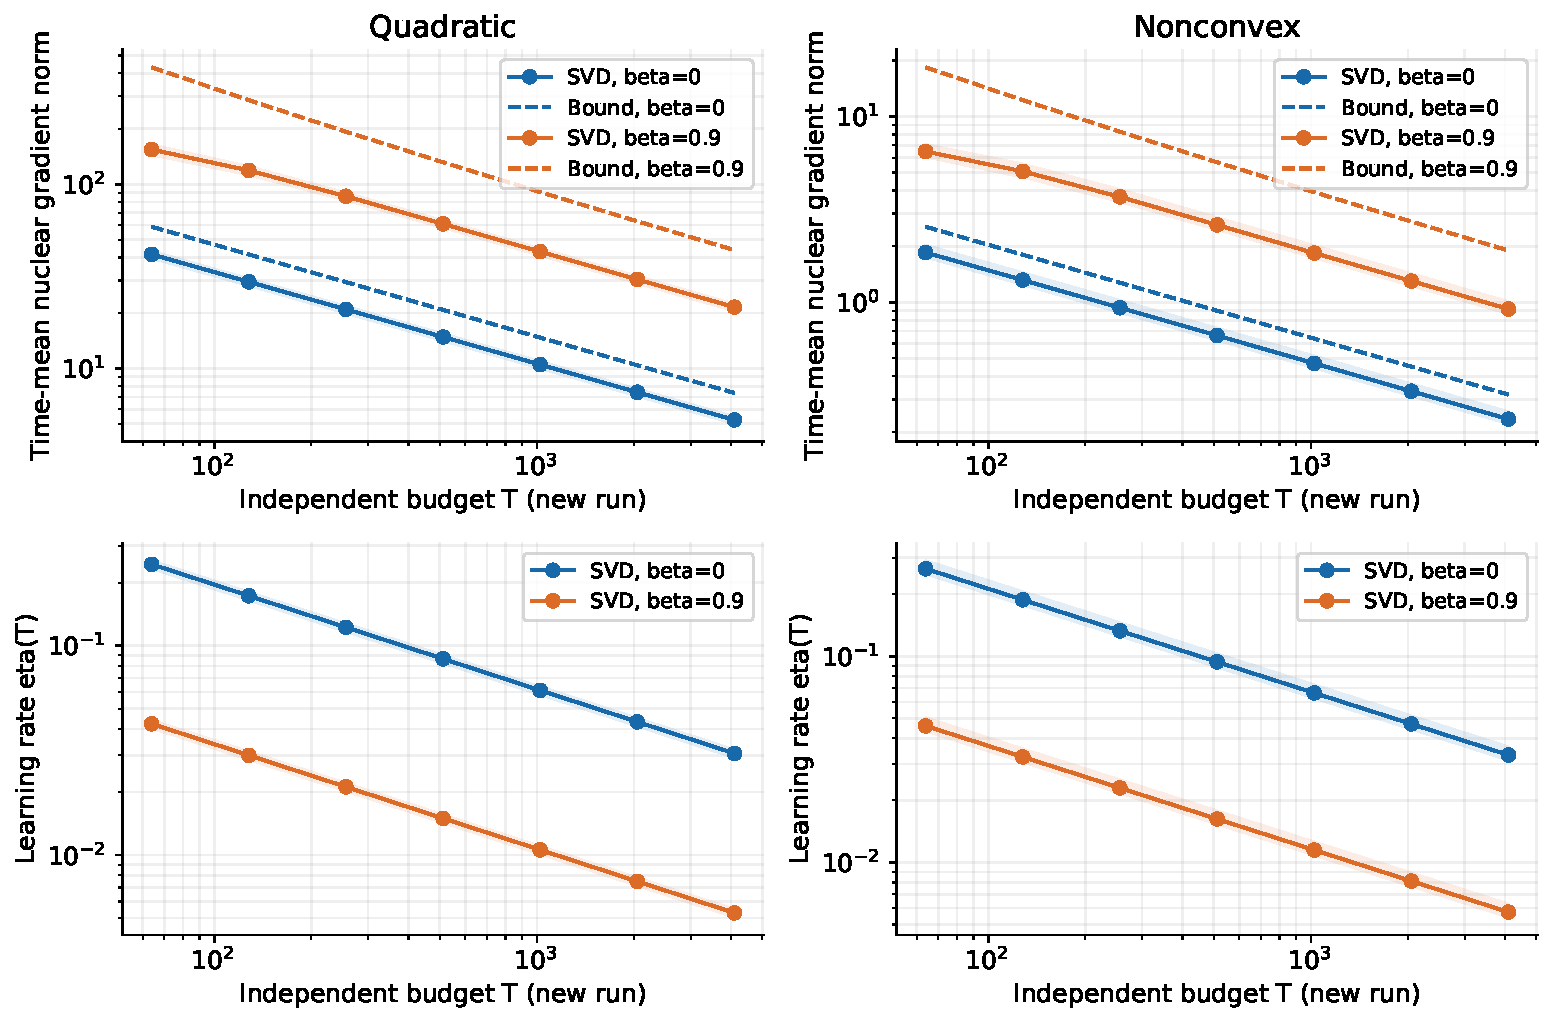
\includegraphics[width=\linewidth]{../results_v2/01_budget_and_learning_rate.pdf}
\caption{重绘原始 \texttt{rates.csv}。上排是时间平均梯度核范数及各自的理论界，下排是每次独立运行实际使用的常学习率。每个点都是重新运行后的统计；上下排共用独立预算 $T$。实线为种子均值，阴影为种子范围。}
\label{fig:budget}
\end{figure}
\textbf{先读坐标。} 上排纵轴不是损失，也不是末步梯度。双对数坐标中，随 $T$ 增大而下降说明更长预算配合更小步长时，时间平均梯度指标变小。虚线是按各自初值计算的理论上界再取种子平均，而不是拟合线。

\textbf{再读数值。} 原有 $2\times2\times\NumSeeds\times7=\NumRuns$ 组运行中，违反上界的次数为 \NumViolations，最大“实测值/上界”为 \MaxRatio。对种子均值做双对数最小二乘拟合，无动量的二次与非凸斜率分别为 \SlopeQuadratic、\SlopeNonconvex；动量对应 \SlopeQuadraticMomentum、\SlopeNonconvexMomentum。它们与这些有限预算中的 $T^{-1/2}$ 趋势相容；有限拟合不能证明一般速率或上界最优性。

\textbf{最后判断可比性。} 下排显示动量组学习率更小，比例见式\eqref{eq:eta-ratio}。例如 $T=2048$ 时，二次问题无动量的种子平均学习率约 0.04327、平均梯度指标约 7.414；动量组对应约 0.007487 和 30.394。后者较高可能包含保守步长造成的早期下降较慢，不能直接说“动量使优化变差”。这张图验证各自的界；下一组图控制学习率后再比较因素。

\subsection{原轨迹：能看步长作用，不能拆出动量或近似的贡献}
\begin{figure}[H]
\centering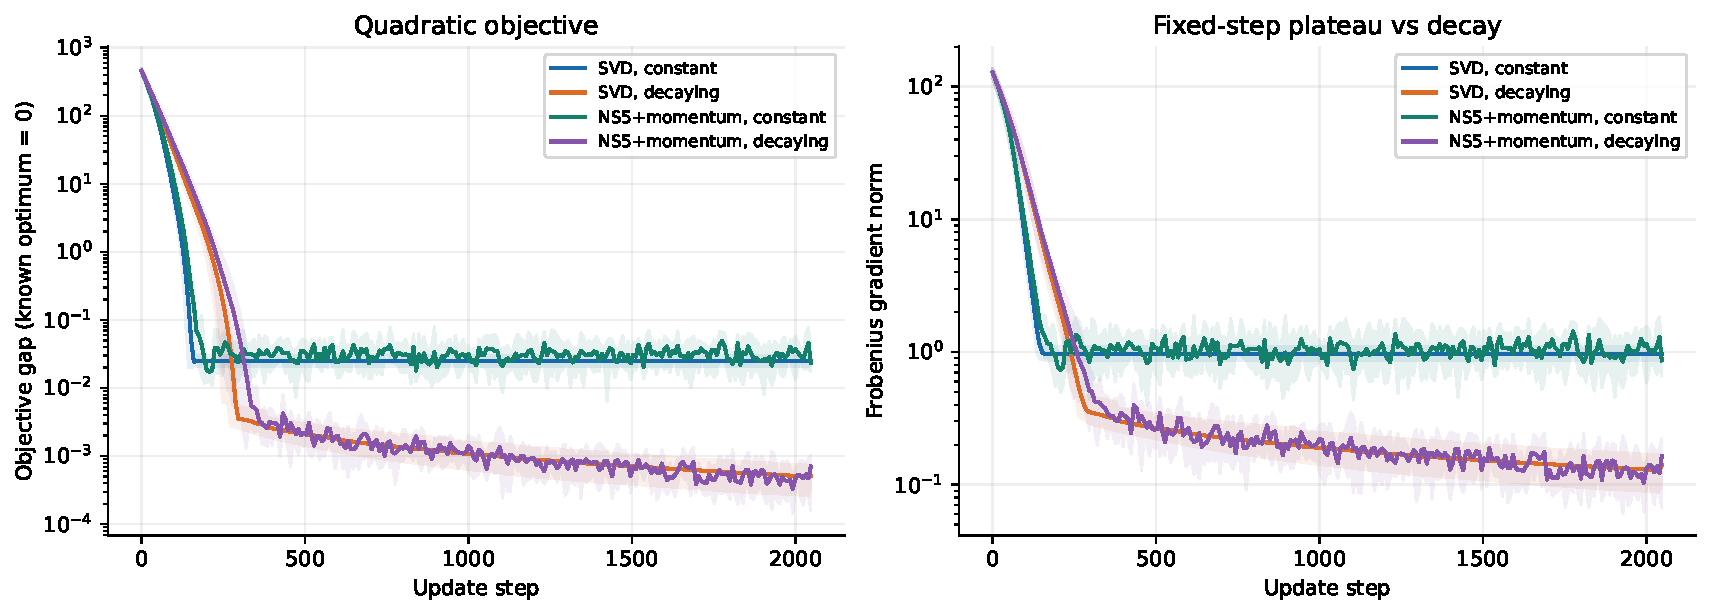
\includegraphics[width=\linewidth]{../results/02_optimization_trajectories.pdf}
\caption{保留原轨迹图。横轴是一次运行内的当前步数；左边为二次目标差，右边为当前梯度 Frobenius 范数。SVD 组无动量，NS5 组带 $\beta=0.9$ 动量；两因素同时改变。}
\label{fig:old-trajectory}
\end{figure}
该图适合在\emph{同一种方法内}对比固定与衰减步长，因为初值、算法和初始步长保持相同，只更换日程。固定 SVD 版本的最终目标差均值为 0.024714，衰减后为 0.000500；NS5 加动量对应 0.037491 和 0.000345。这支持“衰减在本例减小末期误差”，不能从 NS5 与 SVD 的交叉比较中区分动量和近似的作用。

右图显示当前梯度的幅度，不是前图的时间平均核范数。固定步长的正交化更新在梯度变小时未必同步缩短，末期可能跨过最优点；衰减日程缩短位移，因而平台下降。对这一个正定二次目标，函数值差和梯度平方存在 Hessian 特征值控制的联系，但它不是一般非凸目标中可无条件使用的等式。

\subsection{新增受控轨迹：一次只比较一个因素}
\begin{figure}[H]
\centering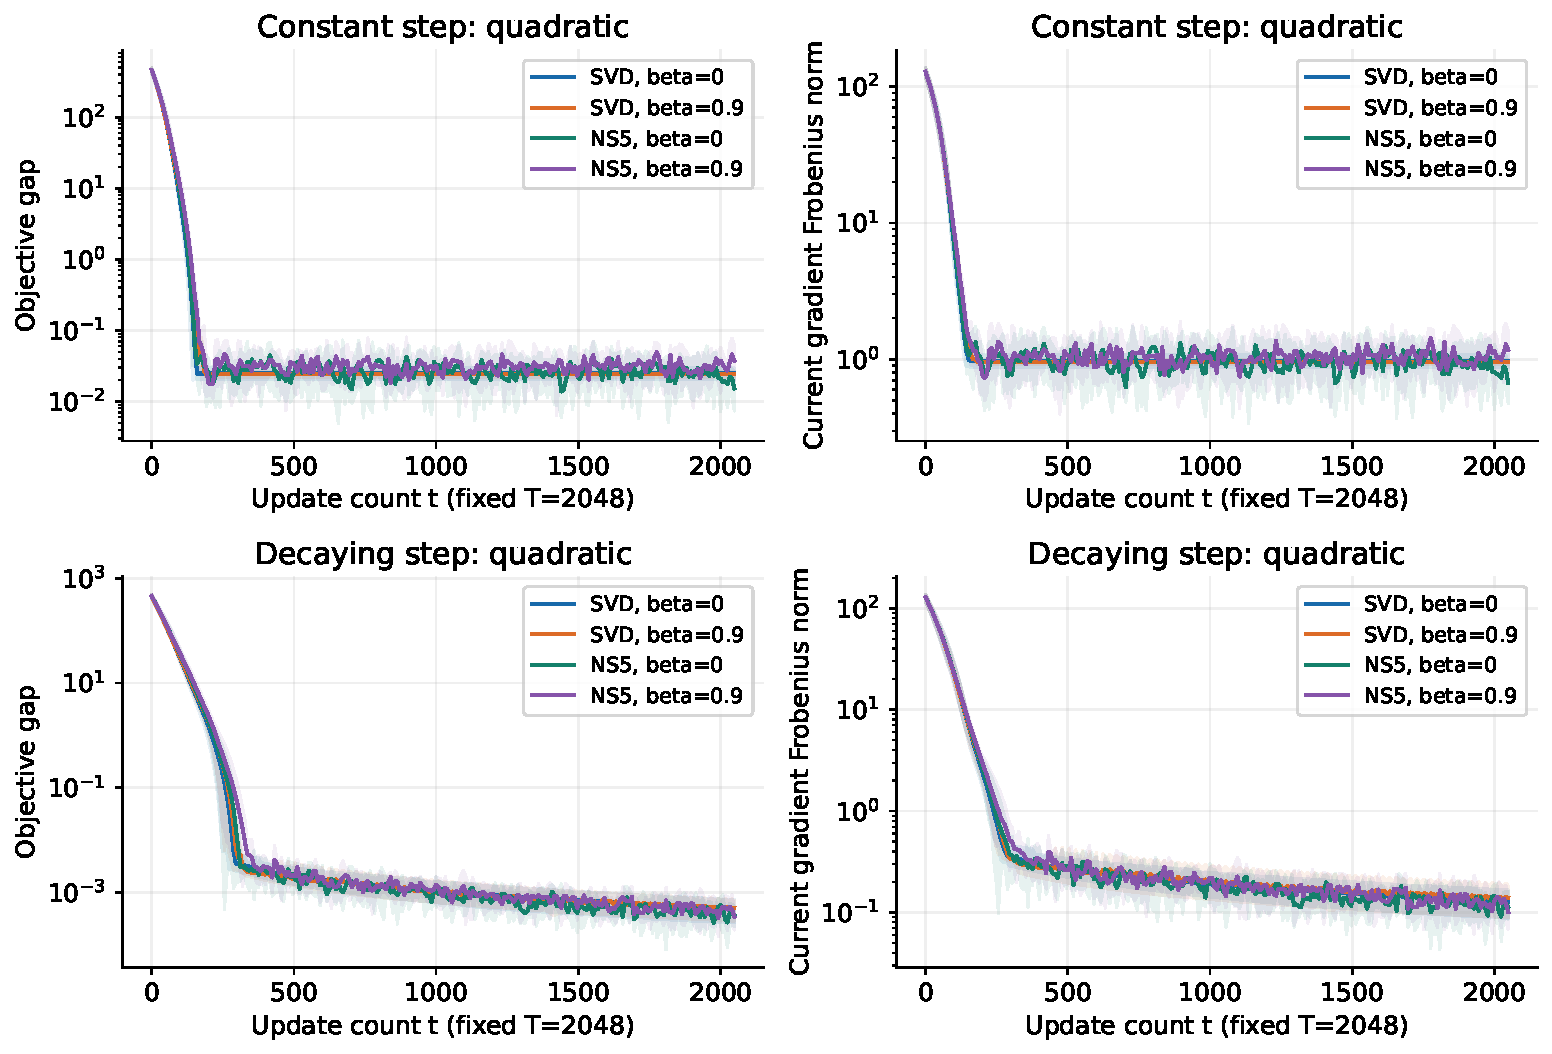
\includegraphics[width=\linewidth]{../results_v2/02_controlled_quadratic.pdf}
\caption{二次目标的受控对照。上排固定学习率，下排衰减学习率；左列目标差，右列当前梯度 Frobenius 范数。每个目标实例内四种方法使用相同日程。蓝/橙固定 SVD 比动量，绿/紫固定 NS5 比动量；蓝/绿固定无动量比近似，橙/紫固定动量比近似。}
\label{fig:controlled-q}
\end{figure}
\begin{figure}[H]
\centering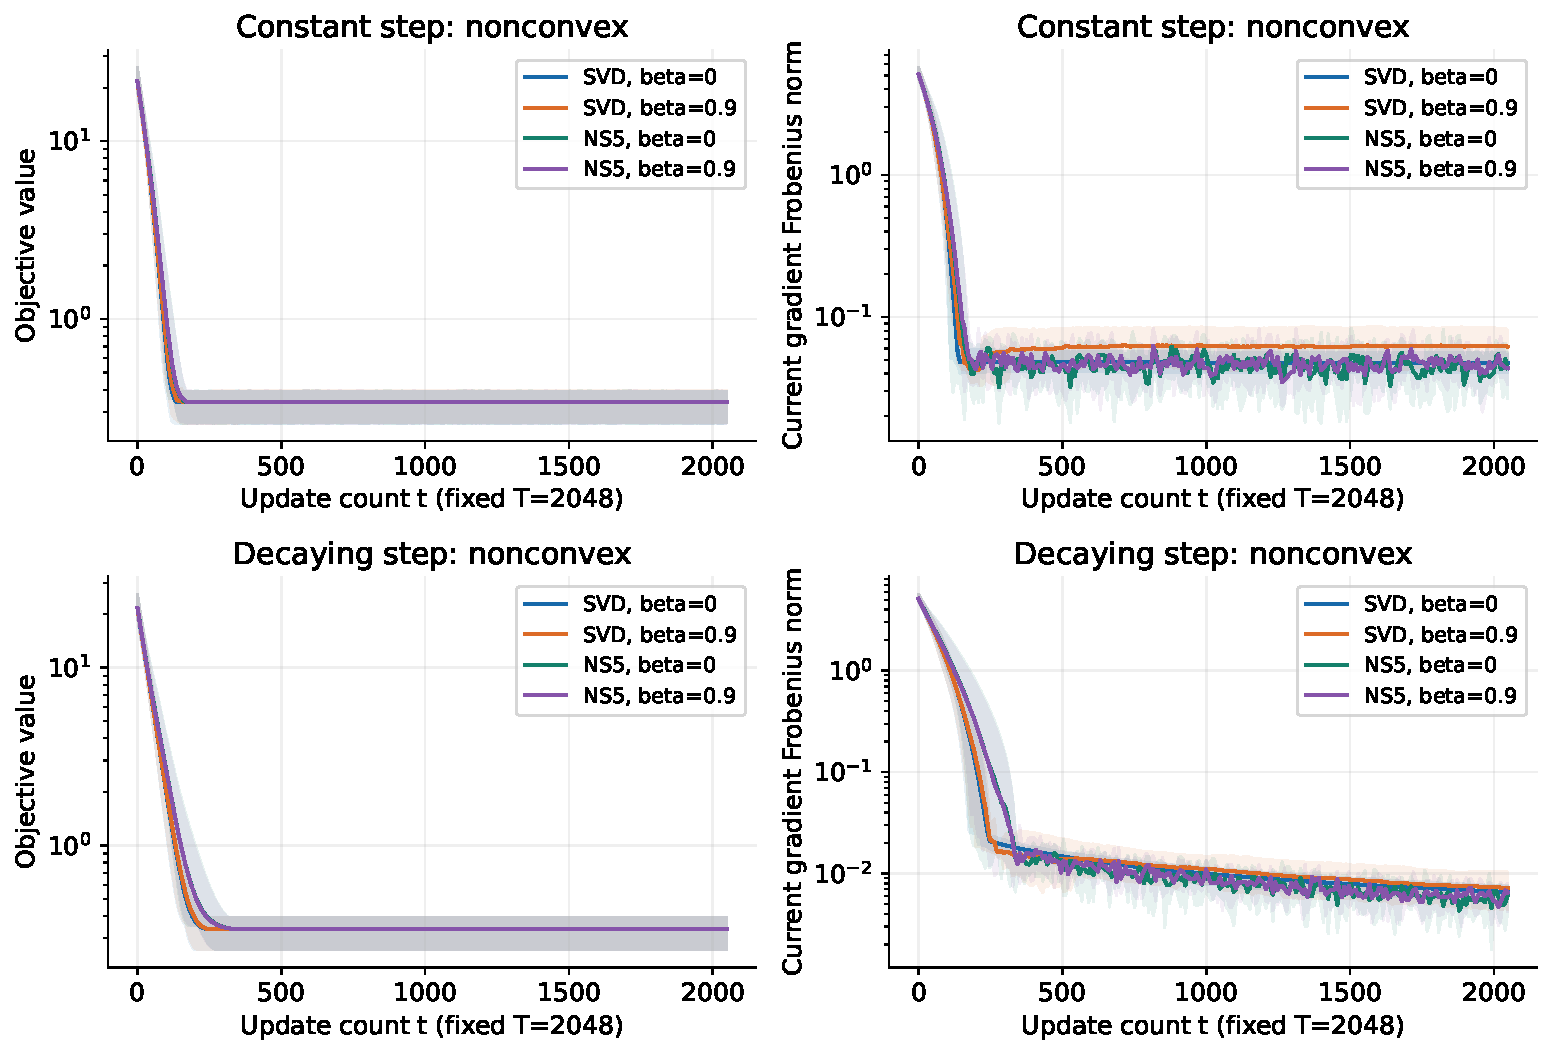
\includegraphics[width=\linewidth]{../results_v2/02_controlled_nonconvex.pdf}
\caption{非凸目标采用与图\ref{fig:controlled-q}相同的对照结构。左列只表示目标值，因为 0 是已知下界，未证明是最优值。$t=2048$ 处显式记录全部更新后的参数。}
\label{fig:controlled-nc}
\end{figure}
\begin{table}[H]
\centering\small
\begin{tabular}{lllrr}
\toprule
目标 & 步长 & 方向与动量 & $f(W_T)$ & $\|G_T\|_\F$\\
\midrule
二次 & 固定 & SVD, $\beta=0$ & 0.024714 & 0.966736\\
二次 & 固定 & SVD, $\beta=0.9$ & 0.024270 & 0.955637\\
二次 & 固定 & NS5, $\beta=0$ & 0.015271 & 0.675672\\
二次 & 固定 & NS5, $\beta=0.9$ & 0.037491 & 1.173654\\
二次 & 衰减 & SVD, $\beta=0$ & 0.000500 & 0.128138\\
二次 & 衰减 & SVD, $\beta=0.9$ & 0.000508 & 0.139911\\
二次 & 衰减 & NS5, $\beta=0$ & 0.000367 & 0.112691\\
二次 & 衰减 & NS5, $\beta=0.9$ & 0.000345 & 0.101095\\
非凸 & 固定 & SVD, $\beta=0$ & 0.339755 & 0.047462\\
非凸 & 固定 & SVD, $\beta=0.9$ & 0.340747 & 0.061676\\
非凸 & 固定 & NS5, $\beta=0$ & 0.339609 & 0.043600\\
非凸 & 固定 & NS5, $\beta=0.9$ & 0.339653 & 0.043653\\
非凸 & 衰减 & SVD, $\beta=0$ & 0.338247 & 0.006582\\
非凸 & 衰减 & SVD, $\beta=0.9$ & 0.338254 & 0.007270\\
非凸 & 衰减 & NS5, $\beta=0$ & 0.338241 & 0.006072\\
非凸 & 衰减 & NS5, $\beta=0.9$ & 0.338245 & 0.006480\\
\bottomrule
\end{tabular}

\caption{80 组新增运行的末步指标，均为五个种子的算术均值；$T=2048$。每行同时列出损失和当前梯度，避免用一个指标替代另一个。}
\label{tab:controlled}
\end{table}
表\ref{tab:controlled}给出可逐项对照的结果。以二次目标为例，固定 SVD 时加入动量后，固定步长的末步目标差由 0.024714 变为 0.024270，变化较小；衰减步长时则由 0.000500 变为 0.000508，没有一致改善。固定 NS5 时，动量在固定步长下将末步目标差从 0.015271 增至 0.037491，而在衰减步长下从 0.000367 降至 0.000345。因而“动量总会降低末期误差”不符合这组受控结果。

固定无动量时，NS5 在二次目标两种日程下的末步目标差都低于 SVD；但固定 $\beta=0.9$ 时，固定步长下 NS5 的 0.037491 高于 SVD 的 0.024270，而衰减下次序反转。这表明近似方法的表现与动量、步长有交互，无法仅由“更接近精确极分解”推出末步损失更低。非凸目标在衰减组中的损失均值均约为 0.33824，而梯度范数仍约为 0.0061--0.0073；目标值接近不意味着驻点性指标完全相同。这些数值是有限种子的描述，未进行显著性检验，不按微小均值差给方法做普遍排名。

共同日程下 NS5 仍与 SVD 有差异，这是方向谱及位移长度改变的综合结果。该受控实验比原图更能定位因素，但没有告诉我们每种方法调参后的最优结果，也没有把步数换算成相同计算预算。在非凸图中，损失和梯度曲线可能以不同尺度下降；驻点性、目标值与最优性仍须分别解释。80 组运行均核查式\eqref{eq:inexact}及逐步下降不等式，验证的是实际误差项被正确纳入。

\subsection{谱图与一维振荡：解释近似和步长的机制}
\begin{figure}[H]
\centering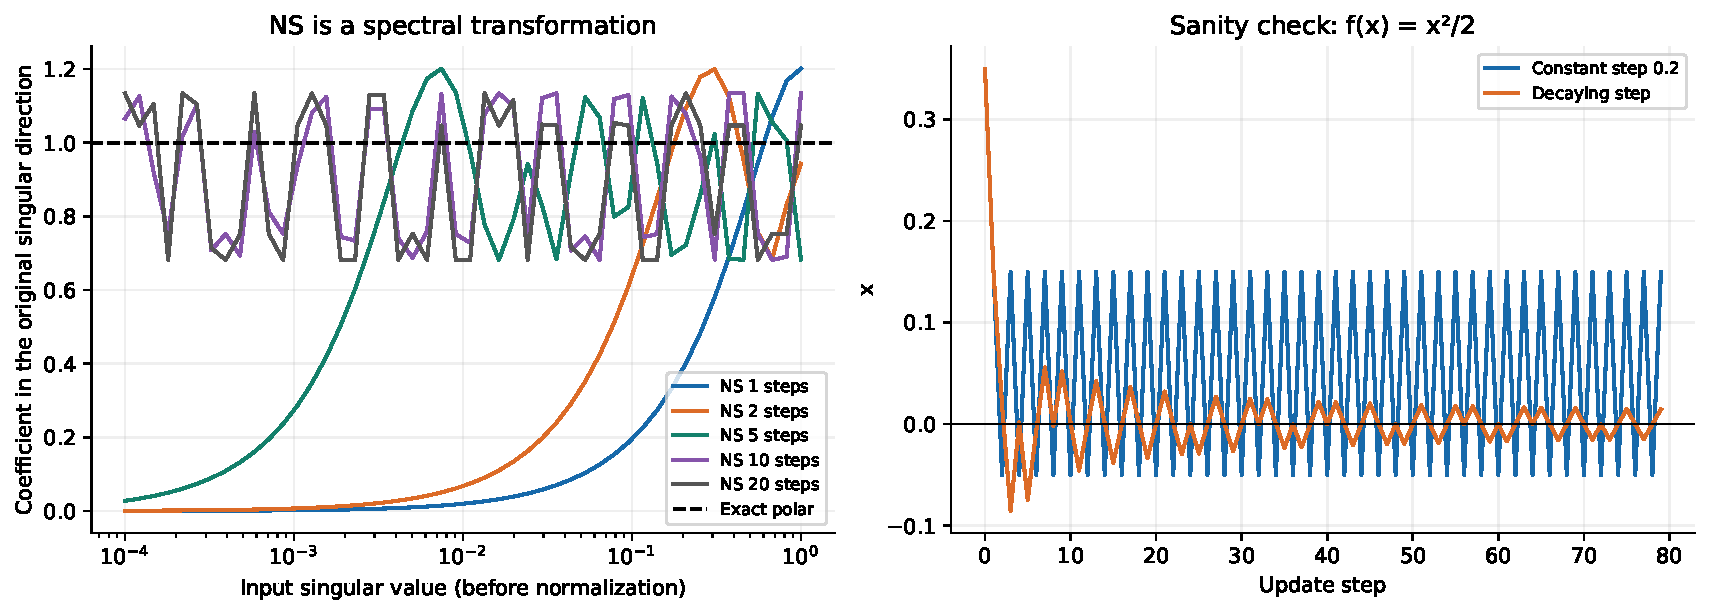
\includegraphics[width=\linewidth]{../results/03_ns_and_step_size.pdf}
\caption{左：同一对角输入的谱变换，固定输入、精度、归一化和系数，仅改变 NS 次数。横轴是归一化前的奇异值；虚线 1 是精确极分解的非零系数。右：固定同一目标 $f(x)=x^2/2$ 与初值，只改变符号更新的步长日程。}
\label{fig:spectrum}
\end{figure}
左图输入为 $\operatorname{diag}(\sigma)$，48 个奇异值按几何序列分布在 $[10^{-4},1]$，条件数为 $10^4$。横轴的值先经整个矩阵的 Frobenius 范数归一化，再参与多项式，不能直接把横轴值当作某次迭代的 $x_{i,j}$。五步对较小奇异方向仍有明显残差；更多步能继续放大这些方向，但已较大的系数也会被多项式改变，故误差不必单调改善。

这里报告的是相对 Frobenius 误差
$\|\operatorname{NS}_K(H)-\Pol(H)\|_\F/\|\Pol(H)\|_\F$。
五步为 \NSFiveError，10 步约 0.202，20 步约 0.215，故“多迭代一定更精确”被该固定输入的结果否定；它也没有说明五步在全部训练输入上误差都等于这个数。与优化轨迹有关的绝对 $\delta_t$ 在控制实验 CSV 中单独记录。

右图在一维取 $x_0=0.35$，精确极分解方向就是 $\operatorname{sign}(x_t)$。固定 $\eta=0.2$ 时，$0.35\to0.15\to-0.05\to0.15$，此后形成二周期。目标是强凸的，方向也精确，但固定长度仍会跨过最小点；这说明观察到平台不等于程序出错。衰减日程在本图中减小了振荡幅度，这一例子不是任意非凸序列收敛的证明。

\subsection{神经网络：阅读两套训练方案的损失}
\begin{figure}[H]
\centering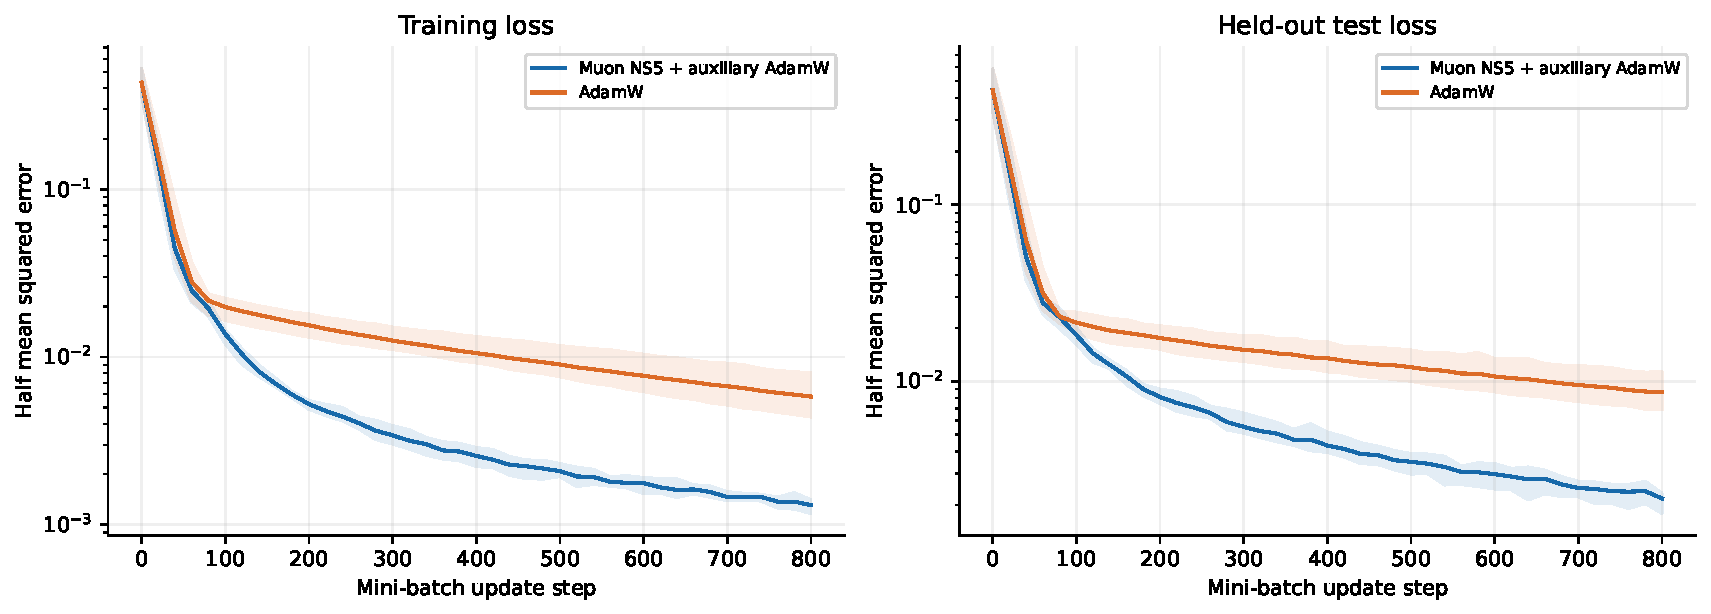
\includegraphics[width=\linewidth]{../results/04_neural_network.pdf}
\caption{原合成回归实验。左为全训练集半均方误差，右为独立测试集半均方误差；横轴是 mini-batch 更新次数，纵轴是损失，未绘制梯度。两方案的隐藏层学习率不同，具体见表\ref{tab:mlp-lr}。阴影为五个种子的范围。}
\label{fig:network}
\end{figure}
第 800 步时，Muon 加辅助 AdamW 的训练/测试损失均值分别为 0.001310/\NeuralMuonTest；全参数 AdamW 对应 0.005808/\NeuralAdamTest。混合方案在这组预设配置中的损失较低。测试损失高于训练损失与存在泛化差距相容；仅凭这两条曲线不能精确分离噪声、样本量与过拟合等因素。

比较时应同时看到：两个方案的隐藏层学习率相差约 6.67 倍、参数组优化器不同，且没有完整超参数搜索。因此这不是在其他条件全部固定时 Muon 对 AdamW 的单因素优势证明，更不能归因为某个动量或 NS 步骤。该网络采用随机 mini-batch、权重衰减及参数分组，不能直接套用前面的全梯度矩阵定理；测试损失下降也没有验证梯度核范数的理论界。

\section{复现、编译与检查}
原版 \texttt{report/muon\_report.tex} 与 PDF 保留；新版为同目录下的 \texttt{muon\_report\_v2.tex} 和 PDF。原 \texttt{results/} 不覆盖，新增控制实验放入 \texttt{results\_v2/}。依赖版本见两版汇总 JSON；无需 GPU、PyTorch 或在线数据集。

在仓库根目录运行：
\begin{verbatim}
python -m pip install -r requirements.txt
OPENBLAS_NUM_THREADS=1 OMP_NUM_THREADS=1 \
  python -m unittest discover -s tests -v
# Reproduce v1 without overwriting the archive
OPENBLAS_NUM_THREADS=1 OMP_NUM_THREADS=1 \
  python -m muon_study.experiments --output /tmp/muon-v1-recheck
# Replot rates.csv and run the 80 controlled experiments
OPENBLAS_NUM_THREADS=1 OMP_NUM_THREADS=1 \
  python -m muon_study.report_v2_experiments --output results_v2
\end{verbatim}
\begin{samepage}
随后进入报告目录，编译两遍以解析交叉引用：
\begin{verbatim}
cd report
xelatex -interaction=nonstopmode -halt-on-error muon_report_v2.tex
xelatex -interaction=nonstopmode -halt-on-error muon_report_v2.tex
\end{verbatim}
\end{samepage}
编译采用 XeLaTeX、Noto Serif/Sans CJK SC 和 DejaVu Sans Mono 字体。原版指标读取 \texttt{results/metrics.tex}；新增表格由 \texttt{controlled\_final.csv} 自动汇总生成，不手抄控制实验数值。自定义种子数或预算后也须同步更新报告中说明的实验配置。

原有 11 项检查覆盖秩亏与零矩阵、极分解恒等式、NS 多项式与转置、动量公式、尺度与衰减、目标有限差分梯度、理论界、全部网络参数组的反向传播以及 AdamW 首步。本次复跑全部通过。原实验在独立目录重跑并与归档数值核对；新增实验对每组同时检查学习率配对、完整终点记录、逐步下降界与加权平均事后界。编译日志、页面与原文件校验结果见 \texttt{results\_v2/VALIDATION.md}。

\begin{table}[H]
\centering\small
\begin{tabularx}{\linewidth}{lX}
\toprule
文件 & 用途\\\midrule
\texttt{muon\_study/optimizers.py} & 原优化器实现，本版继续调用\\
\texttt{muon\_study/report\_v2\_experiments.py} & 新版预算重绘、受控实验、检查与表格导出\\
\texttt{results/rates.csv} & 原始 140 组预算实验及各组学习率\\
\texttt{results\_v2/controlled\_trajectories.csv} & 当前目标、梯度、学习率、方向内积及误差\\
\texttt{results\_v2/controlled\_final.csv} & 每组 $W_T$ 指标与含误差的事后界\\
\texttt{results\_v2/summary.json} & 新版环境版本及 80 组控制实验汇总\\
\bottomrule
\end{tabularx}
\caption{新增原始数据与报告的对应关系。}
\end{table}

\noindent\textbf{GitHub：}
\url{https://github.com/rou521/optimize-and-game}。
\href{https://github.com/rou521/optimize-and-game/blob/main/report/muon_report_v2.tex}{新版 TeX}、
\href{https://github.com/rou521/optimize-and-game/blob/main/report/muon_report_v2.pdf}{新版 PDF}、
\href{https://github.com/rou521/optimize-and-game/blob/main/muon_study/report_v2_experiments.py}{新增实验脚本}。
完整工程可用仓库的 \texttt{Code} $\to$ \texttt{Download ZIP}，或
\href{https://github.com/rou521/optimize-and-game/archive/refs/heads/main.zip}{工程 ZIP 链接}下载。
\texttt{SHA256SUMS.json} 保存文件校验值；GitHub 文件页按 \texttt{y} 可获得固定提交链接。

\section{结论}
损失规定训练的目标，梯度将目标变成局部变化信息，内积衡量给定更新的一阶收益，范数控制幅度与曲率成本。SVD 将矩阵方向和强度分开，精确 Muon 将正奇异值重置为 1，因而同时获得核范数收益与有界位移。动量引入历史信息及跟踪误差，有限步 NS 用矩阵乘法完成近似谱变换并留下近似误差。沿这条链条，精确版本的有限预算证明与实际算法的差别都可以逐项定位。

在明示的全梯度条件下，精确版本及固定动量版本有时间平均梯度的 $O(T^{-1/2})$ 上界。独立预算图用于核查这一命题；同学习率的控制轨迹用于区分因素；谱图解释近似残差；小型网络展示两套完整训练方案的损失表现。四类证据各有用途，均不能单独扩展为随机大模型训练的普遍收敛或优越性结论。

\clearpage
\begin{thebibliography}{9}
\raggedright
\bibitem{jordan} Keller Jordan, Yuchen Jin, Vlado Boza, You Jiacheng, Franz Cesista, Laker Newhouse, Jeremy Bernstein.
\emph{Muon: An optimizer for hidden layers in neural networks}. 2024.
\url{https://github.com/KellerJordan/Muon}.
算法简介与引用信息依据作者仓库 README。
\bibitem{liu} Jingyuan Liu, Jianlin Su, Xingcheng Yao, et al.
\emph{Muon is Scalable for LLM Training}. 2025. arXiv:2502.16982.
\url{https://arxiv.org/abs/2502.16982}.
本文阅读的原文来自
\href{https://github.com/MoonshotAI/Moonlight/blob/c2ad5b20c605086526a179d36901bfc41b52b44b/Moonlight.pdf}{MoonshotAI/Moonlight 作者仓库的论文 PDF（固定版本）}。
\bibitem{code} Keller Jordan et al. \emph{Muon reference implementation: muon.py}.
固定提交：\nolinkurl{f98f1cacc0263b04290753e32be8d498c1efc806}。
\href{https://github.com/KellerJordan/Muon/blob/f98f1cacc0263b04290753e32be8d498c1efc806/muon.py}{GitHub：Muon 固定版本源码}。
\end{thebibliography}
\end{document}
